\documentclass[aspectratio=169]{beamer}\usepackage[]{graphicx}\usepackage[]{color}
% maxwidth is the original width if it is less than linewidth
% otherwise use linewidth (to make sure the graphics do not exceed the margin)
\makeatletter
\def\maxwidth{ %
  \ifdim\Gin@nat@width>\linewidth
    \linewidth
  \else
    \Gin@nat@width
  \fi
}
\makeatother

\definecolor{fgcolor}{rgb}{0.345, 0.345, 0.345}
\newcommand{\hlnum}[1]{\textcolor[rgb]{0.686,0.059,0.569}{#1}}%
\newcommand{\hlstr}[1]{\textcolor[rgb]{0.192,0.494,0.8}{#1}}%
\newcommand{\hlcom}[1]{\textcolor[rgb]{0.678,0.584,0.686}{\textit{#1}}}%
\newcommand{\hlopt}[1]{\textcolor[rgb]{0,0,0}{#1}}%
\newcommand{\hlstd}[1]{\textcolor[rgb]{0.345,0.345,0.345}{#1}}%
\newcommand{\hlkwa}[1]{\textcolor[rgb]{0.161,0.373,0.58}{\textbf{#1}}}%
\newcommand{\hlkwb}[1]{\textcolor[rgb]{0.69,0.353,0.396}{#1}}%
\newcommand{\hlkwc}[1]{\textcolor[rgb]{0.333,0.667,0.333}{#1}}%
\newcommand{\hlkwd}[1]{\textcolor[rgb]{0.737,0.353,0.396}{\textbf{#1}}}%
\let\hlipl\hlkwb

\usepackage{framed}
\makeatletter
\newenvironment{kframe}{%
 \def\at@end@of@kframe{}%
 \ifinner\ifhmode%
  \def\at@end@of@kframe{\end{minipage}}%
  \begin{minipage}{\columnwidth}%
 \fi\fi%
 \def\FrameCommand##1{\hskip\@totalleftmargin \hskip-\fboxsep
 \colorbox{shadecolor}{##1}\hskip-\fboxsep
     % There is no \\@totalrightmargin, so:
     \hskip-\linewidth \hskip-\@totalleftmargin \hskip\columnwidth}%
 \MakeFramed {\advance\hsize-\width
   \@totalleftmargin\z@ \linewidth\hsize
   \@setminipage}}%
 {\par\unskip\endMakeFramed%
 \at@end@of@kframe}
\makeatother

\definecolor{shadecolor}{rgb}{.97, .97, .97}
\definecolor{messagecolor}{rgb}{0, 0, 0}
\definecolor{warningcolor}{rgb}{1, 0, 1}
\definecolor{errorcolor}{rgb}{1, 0, 0}
\newenvironment{knitrout}{}{} % an empty environment to be redefined in TeX

\usepackage{alltt}
\usepackage{multirow}
%\usecolortheme{beaver}
%\usecolortheme[RGB={129,3,3}]{structure}
\usetheme{CambridgeUS}
\usecolortheme{seahorse}

% Standard header (will need to change date!)
\title[GEOG 5680 Summer '20]{GEOG 5680\\Introduction to R}
\subtitle[Intro]{02: Variables in R}
\author[S. Brewer]{Simon Brewer}
\institute[Univ. Utah]{
  Geography Department\\
  University of Utah\\
  Salt Lake City, Utah 84112\\[1ex]
  \texttt{simon.brewer@geog.utah.edu}
}
\date[May 02, 2020]{May 02, 2020}
\IfFileExists{upquote.sty}{\usepackage{upquote}}{}
\begin{document}



%--- the titlepage frame -------------------------%
\begin{frame}
  \titlepage
\end{frame}

% \section{Objectives}
% %--- Slide 3 ----------------%
% \begin{frame}{Objectives}
% \begin{itemize}
%   \item The R environment
%   \item R variables
%   \item Creating variables in R ``on the fly''
%   \item Different object types
%   \item Importing and exporting from files
% \end{itemize}
% \end{frame}
% 
% \section{The R Environment}
% %--- Slide ----------------%
% \begin{frame}{The R Environment}
% \begin{columns}
% 	\begin{column}{0.29\textwidth}
% 	Starting R
% 	\begin{itemize}
% 		\item Windows --- R icon
% 		\item Mac OSX --- Applications $>$ R
% 		\item Unix --- Terminal $>$ R
%     \item \textbf{Or use RStudio!}
% 	\end{itemize}
% 	\end{column}
% 	\begin{column}{0.69\textwidth}
% 		\begin{center}
% 			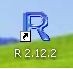
\includegraphics[width=0.25\textwidth]{./images/Ricon.png}
% 			~
% 			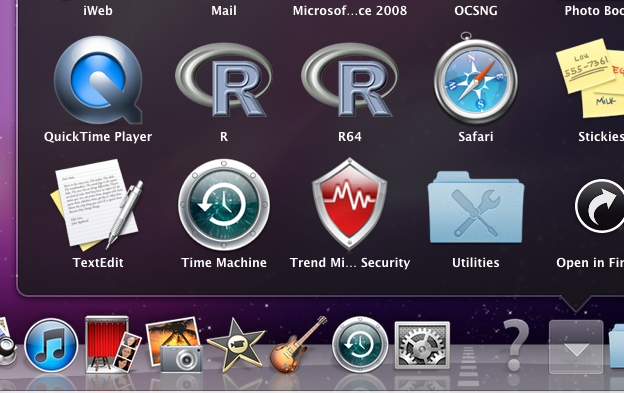
\includegraphics[width=0.375\textwidth]{./images/macApps.png}
% 			~
% 			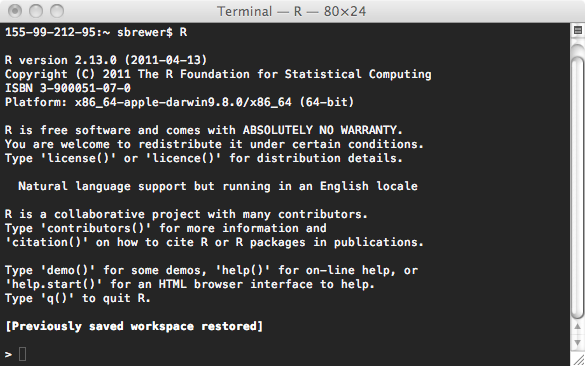
\includegraphics[width=0.375\textwidth]{./images/terminalR.png}\\
% 			\smallskip
% 			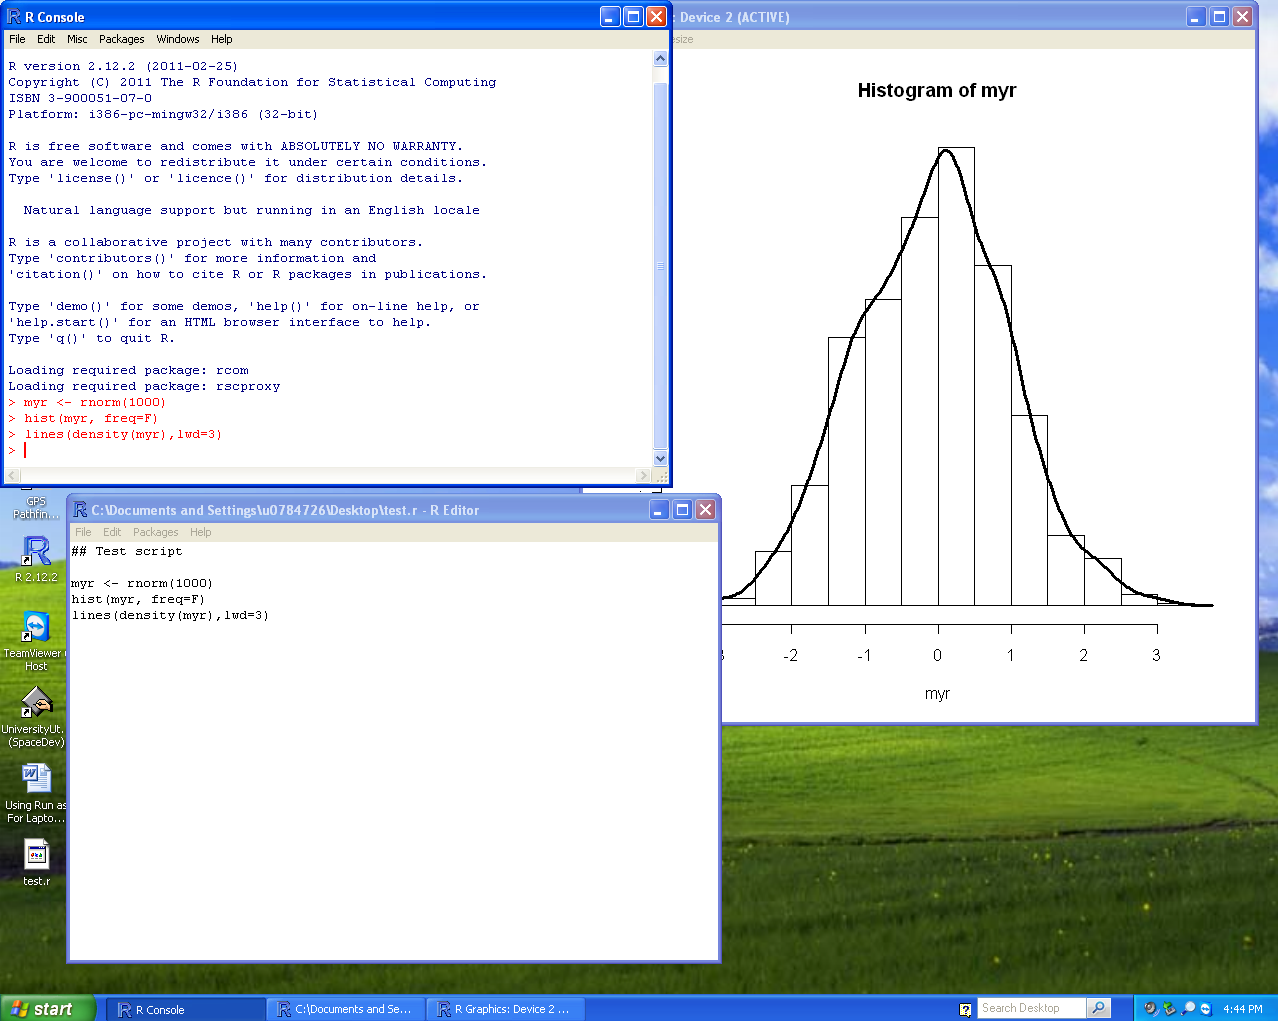
\includegraphics[width=0.5\textwidth]{./images/RworkspaceWin.PNG}
% 			~
% 			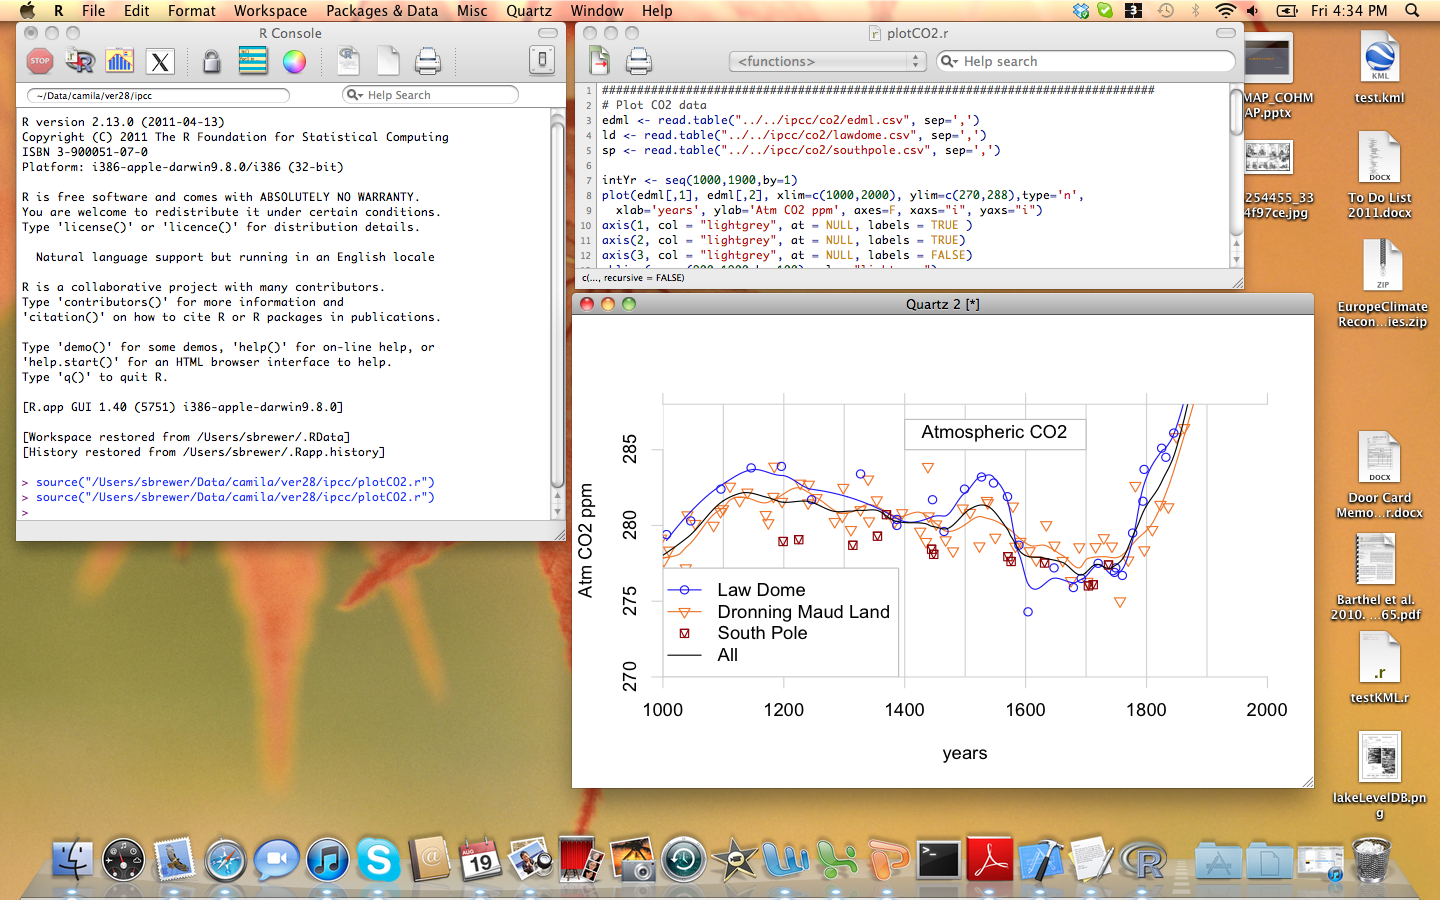
\includegraphics[width=0.5\textwidth]{./images/RworkspaceMac.png}
% 
% 		\end{center}
% 	\end{column}
% \end{columns}
% 
% \end{frame}
% 
%--- Slide ----------------%
\begin{frame}{The R Environment}
\begin{columns}
	\begin{column}{0.5\textwidth}
  \begin{itemize}
		\item The working directory
    \begin{itemize}
      \item The directory R is currently running in
      \item Affects access to files, etc
  		\item When you start R, it will generally start in a root directory
      \item Change R to directory where you store your files
      \item 'Session' menu --- 'Set working directory'
      \item Can also be set from the 'Files' tab

    \end{itemize}
	\end{itemize}
	\end{column}
	\begin{column}{0.5\textwidth}
	\begin{itemize}
		\item<2-> The workspace
    \begin{itemize}
      \item<2-> R's memory
      \item<2-> Variables and data are held here during a session
      \item<2-> Note that you are not altering the contents of a file as you work (c.f. Excel, etc)
      \item<2-> Can cause some limitations on data size
    \end{itemize}
	\end{itemize}
	\end{column}
\end{columns}

\end{frame}

% %--- Slide ----------------%
% \begin{frame}{The R Environment}
%   \begin{itemize}
% 		\item The working directory
%     \begin{itemize}
%       \item The directory R is currently running in
%       \item Affects access to files, etc
%   		\item When you start R, it will generally start in a root directory
%       \item Change R to directory where you store your files
%       \item 'Session' menu --- 'Set working directory'
%       \item Can also be set from the 'Files' tab
% 
%     \end{itemize}
% 	\end{itemize}
% \end{frame}
% 
% %--- Slide ----------------%
% \begin{frame}{The R Environment}
% 	\begin{itemize}
% 		\item The workspace
%     \begin{itemize}
%       \item R's memory
%       \item Variables and data are held here during a session
%       \item Note that you are not altering the contents of a file as you work (c.f. Excel, etc)
%       \item Can cause some limitations on data size
%     \end{itemize}
% 	\end{itemize}
% \end{frame}
% 
% % %--- Slide ----------------%
% \begin{frame}{Variables in R}
% \begin{itemize}
%   \item All data is read in and stored in memory for analysis in objects or variables
%   \item A name and a value: \texttt{x <- 5}
%   \item Modes
% 		\begin{itemize}
% 			\item Numeric		e.g. 5 or 6e-5	
% 			\item Character	e.g. ``Green'' or ``Red''
% 			\item Factor		e.g. classes: ``male'' ``female''
% 			\item Logic		True/False
% 		\end{itemize}
% 	\item Classes
% 		\begin{itemize}
% 			\item Vector	---	1-dimensional
% 			\item Matrix --- 2-dimensional
% 			\item Array	---	Multi-dimensional
% 			\item Data frame ---	2-dimensional with different modes
% 			\item List 	---	set of other objects
% 		\end{itemize}
%     \item Variables do not need to be declared (c.f. C++, Fortran)
% 	\end{itemize}
% \end{frame}
% 
% %--- Slide ----------------%
% \begin{frame}{The R Environment}
% \begin{columns}
% 	\begin{column}{0.40\textwidth}
% 	\begin{itemize}
% 		\item Recalling commands --- Arrow keys let you cycle through previous commands
% 		\item Stopping R
% 		\begin{itemize}
% 		  \item \texttt{q()}
% 		  \item Save session?
% 		  \item .Rhistory .Rdata files 
% 		\end{itemize}
% 	\end{itemize}
% 	\end{column}
% 	\begin{column}{0.59\textwidth}
% 		\begin{center}
% 			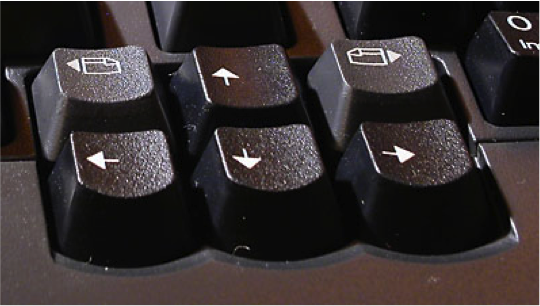
\includegraphics[width=0.74\textwidth]{./images/arrowkeys.png}\\
% 			\smallskip
% 			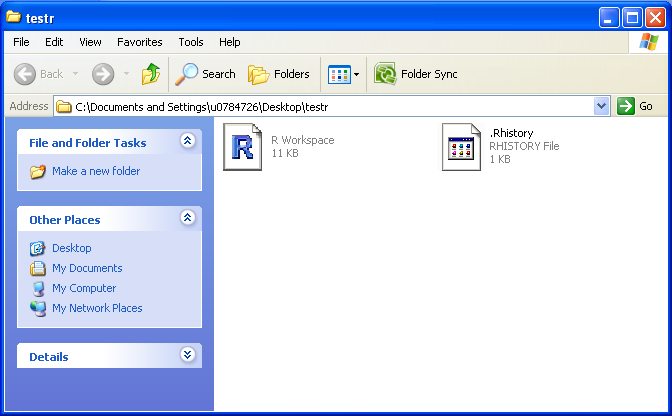
\includegraphics[width=0.74\textwidth]{./images/rdata.png}
% 
% 		\end{center}
% 	\end{column}
% \end{columns}
% \end{frame}
% 
\section{Variables in R}
%--- Slide ----------------%
\begin{frame}{Variables in R}
\begin{itemize}
  \item All data is read in and stored in memory for analysis
  \item Variables are \emph{objects} used to store data
  \item A variable consists of a name and a value \emph{that can be changed}:
		\begin{itemize}
			\item  \texttt{x <- 5}
			\item Creates a variable $x$ with the value 5
			\item  \texttt{x <- 10}
			\item Changes the value of $x$ to 10
			\item  \texttt{x <- x + 10}
			\item Changes the value of $x$ to 20
		\end{itemize}
	\end{itemize}
\end{frame}

%--- Slide ----------------%
\begin{frame}{Variables in R}
\begin{itemize}
	\item Variables have different modes and classes
	\item Modes
		\begin{itemize}
			\item Numeric:		e.g. 5 or 6e-5	
			\item Character:	e.g. ``Green'' or ``Red''
			\item Factor (categories):		e.g. ``male'' ``female''
			\item Logic:		True/False
		\end{itemize}
	\item Classes
		\begin{itemize}
			\item Scalar/Vector/Matrix/Array/Data frame/List
		\end{itemize}
	\end{itemize}
\end{frame}

%--- Slide ----------------%
\begin{frame}{Variables in R}
\begin{columns}
  \begin{column}{0.50\textwidth}
		\begin{itemize}
  		\item \textbf{Simple variable/scalar}
		  \item No dimension, no index
		  \item E.g. population of Salt Lake City
		\end{itemize}
		\begin{center}
			
\includegraphics[width=0.1\textwidth]{./images/nod_variable.png}
		\end{center}
	\end{column}
	\begin{column}{0.50\textwidth}
		\begin{itemize}
  		\item \textbf{Vector}
		  \item One dimension, one index $[i]$
		  \item Same mode
		  \item E.g. series of monthly temperature
		\end{itemize}
		\begin{center}
			
\includegraphics[width=0.25\textwidth]{./images/1d_vector.png}
		\end{center}
	\end{column}
\end{columns}
\end{frame}

%--- Slide ----------------%
\begin{frame}{Variables in R}
\begin{columns}
  \begin{column}{0.50\textwidth}
		\begin{itemize}
  		\item \textbf{Matrix}
		  \item Two dimensions, two indices $[i,j]$
		  \item Same mode
		  \item E.g. gridded climate or raster image
		\end{itemize}
		\begin{center}
      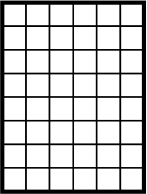
\includegraphics[width=0.25\textwidth]{./images/2d_matrix.png}
		\end{center}
	\end{column}
	\begin{column}{0.50\textwidth}
		\begin{itemize}
  		\item \textbf{Array}
		  \item $n$ dimension, $n$ indices $[i,j,\ldots]$
		  \item Same mode
		  \item E.g. set of remote sensed images over time
		\end{itemize}
		\begin{center}
			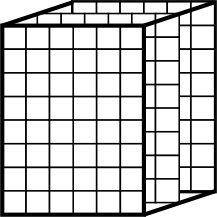
\includegraphics[width=0.25\textwidth]{./images/3d_array.png}
		\end{center}
	\end{column}
\end{columns}
\end{frame}

%--- Slide ----------------%
\begin{frame}{Variables in R}
\begin{columns}
	\begin{column}{0.50\textwidth}
		\begin{itemize}
  		\item \textbf{Data frame}
		  \item 2 dimensions, 2 indices $[i,j]$ or by name (\texttt{\$})
		  \item \textbf{Different} modes
		  \item Most study data, e.g. census data (income class, household size), 
		\end{itemize}
		\begin{center}
			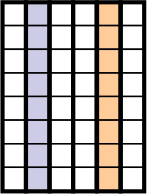
\includegraphics[width=0.4\textwidth]{./images/2d_dataframe.png}\\
		\end{center}
	\end{column}
	\begin{column}{0.50\textwidth}
		\begin{itemize}
  		\item \textbf{List}
		  \item Set of different objects, index by object name (\texttt{\$})
		  \item Frequently output from R functions --- e.g. regression model may have coefficients, R$^2$, residuals
		\end{itemize}
		\begin{center}
			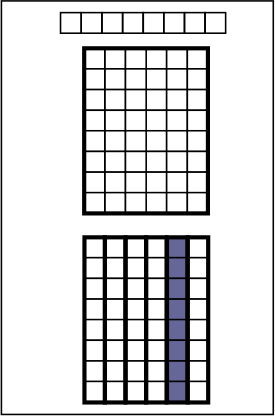
\includegraphics[width=0.45\textwidth]{./images/list.png}
		\end{center}
	\end{column}
\end{columns}
\end{frame}

% %--- Slide ----------------%
% \begin{frame}{Importing/exporting data}
% 	\begin{itemize}
% 		\item Variables can be created `on-the-fly' in R
%     \item More commonly use ASCII text files to import as data frame
%     \item Comma separated (CSV) files are simple way to transfer between Excel and R
%     \item Add-on packages for other formats
%     \begin{itemize}
%       \item NetCDF, raster images
%       \item Specialized outout (e.g. sequencing, json)
%       \item Databases, incl. Excel (ODBC)
%       \item Most image formats
%     \end{itemize}
% 	\end{itemize}
% \end{frame}
% 
% \section{Functions in R}
% %--- Slide ----------------%
% \begin{frame}{Functions in R}
% \begin{itemize}
%   \item What is a function?
% 	\begin{itemize}
% 		\item Any operation			
% 		\item Either on some data: \texttt{sqrt(9)} --- returns square root of nine
% 		\item Or on the system: \texttt{ls()} --- returns list of objects in R's memory
% 		%\item Note parentheses
% 		\item Parantheses used to provide the variable or data name 
% 		\begin{itemize}
%       \item Also used to specify options --- modify the functions behavior
%     \end{itemize}
%   \end{itemize}
% \end{itemize}
% \end{frame}
% 
% %--- Slide ----------------%
% \begin{frame}{Functions in R}
% \begin{itemize}
% 	\item Some basic functions
% 	\begin{itemize}
% 		\item  \texttt{min(sl);  max(sl) ;  sum(sl)}
% 		\item  \texttt{mean(sl) ; sd(sl) ; var(sl) ; median(sl)}
% 		\item  \texttt{quantile(sl, 0.5) ; range(sl)}
% 		\item  \texttt{summary(sl)}
% 		\item  \texttt{levels(sp)}
% 		\item  \texttt{table(sp)}
% 	\end{itemize}
% \end{itemize}
% \end{frame}
%' 
%' %--- Slide ----------------%
%' \begin{frame}[fragile]{Functions in R}
%' Functions adapt to data classes: \texttt{summary} with a vector
%' <<>>=
%' summary(iris$Sepal.Length)
%' @
%' \end{frame}
%' 
%' %--- Slide ----------------%
%' \begin{frame}[fragile]{Functions in R}
%' Functions adapt to data classes: \texttt{summary} with factors
%' <<>>=
%' summary(iris$Species)
%' @
%' \end{frame}
%' 
%' %--- Slide ----------------%
%' \begin{frame}[fragile]{Functions in R}
%' Functions adapt to data classes: \texttt{summary} with a data frame
%' <<>>=
%' summary(iris)
%' @
%' \end{frame}
%' 
%' 
%' %--- Slide ----------------%
%' \begin{frame}{Functions in R}
%' \begin{itemize}
%' 	\item Assignment (\texttt{<-} or \texttt{=}) to store output in new variable
%' 	\begin{itemize}
%' 		\item  \texttt{y <- sqrt(5)}
%' 	\end{itemize}
%' 	\item<2-> Output can be used in new functions
%' 	\begin{itemize}
%' 		\item  \texttt{round(y)}
%' 	\end{itemize}
%'   \item<3-> Functions can be combined
%' 	\begin{itemize}
%' 		\item  \texttt{round(sqrt(5))}
%' 	\end{itemize}
%' 	\item<4-> Options (what goes in the parentheses):
%' 	\begin{itemize}
%' 		\item \texttt{seq(from=0,to=20,by=2)} or \texttt{seq(0,20,2)}
%' 	\end{itemize}
%' 	\item<5-> A function is an object --- can easily be created
%' 	\begin{itemize}
%' 		\item  \texttt{mySD <- function(x) \{ sqrt(var(x))\}}
%' 		\item \texttt{mySD(sl)}
%' 		%\item Compare to: \texttt{sd(sl)}
%' 	\end{itemize}
%' \end{itemize}
%' \end{frame}
%' 
%' %--- Slide ----------------%
%' \begin{frame}{Functions in R}
%' \begin{itemize}
%' 	\item Getting help with functions
%' 	\begin{itemize}
%' 		\item  \texttt{help()}
%'   	\item  \texttt{help(mean)}
%'   	\item  \texttt{?mean}
%' 	\end{itemize}
%' 	\item Gives brief explanation of function plus information on the parameters, data input and resulting output
%' 	\item Help browser
%' \end{itemize}
%'   	\begin{center}
%' 			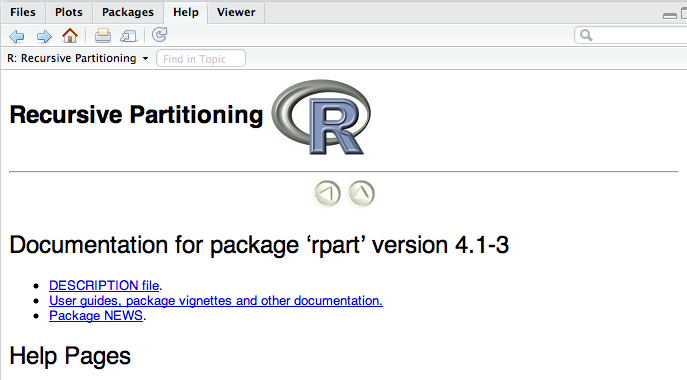
\includegraphics[width=0.5\textwidth]{./images/help1.png}\\
%' 		\end{center}
%' \end{frame}


% %--- Slide 20 ----------------%
% \begin{frame}{Next Class}
% \begin{itemize}
% 	\item Lab: variable creation and data import/export
% 	\item 0102: Accessing subsets of data and variables
% \end{itemize}
% \end{frame}

\end{document}
